%!TEX root = ../main.tex
\subsection{Fake versus real normals}
\label{s:results:normals}

\begin{figure}
	\centering
	\begin{subfigure}[t]{0.32\linewidth}
		\centering
		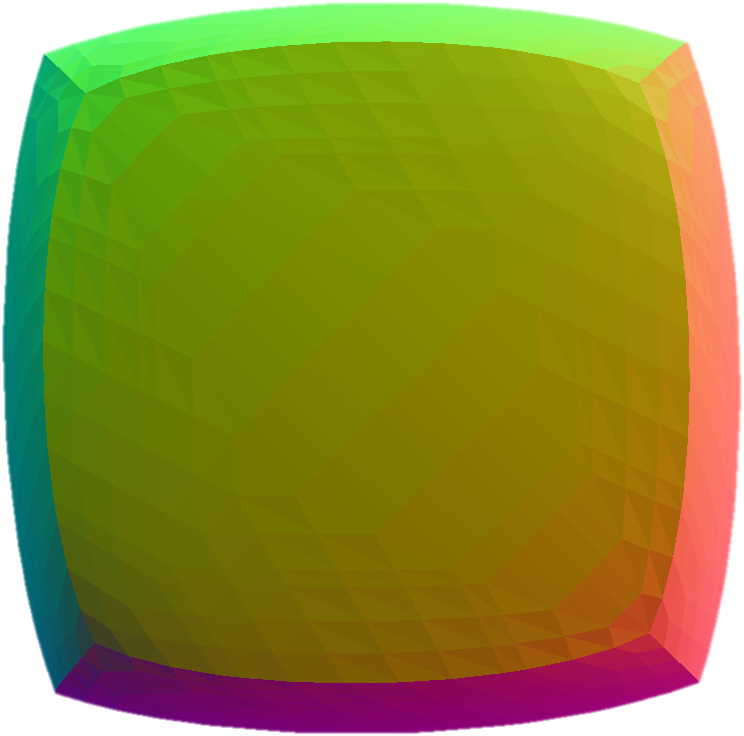
\includegraphics[width=\textwidth]{content/img/results/normals/cubeFakeNormals.png}
		\caption{`Fake' normals}
		\label{fig:results:normals:original:fake}
	\end{subfigure}
	\begin{subfigure}[t]{0.32\linewidth}
		\centering
		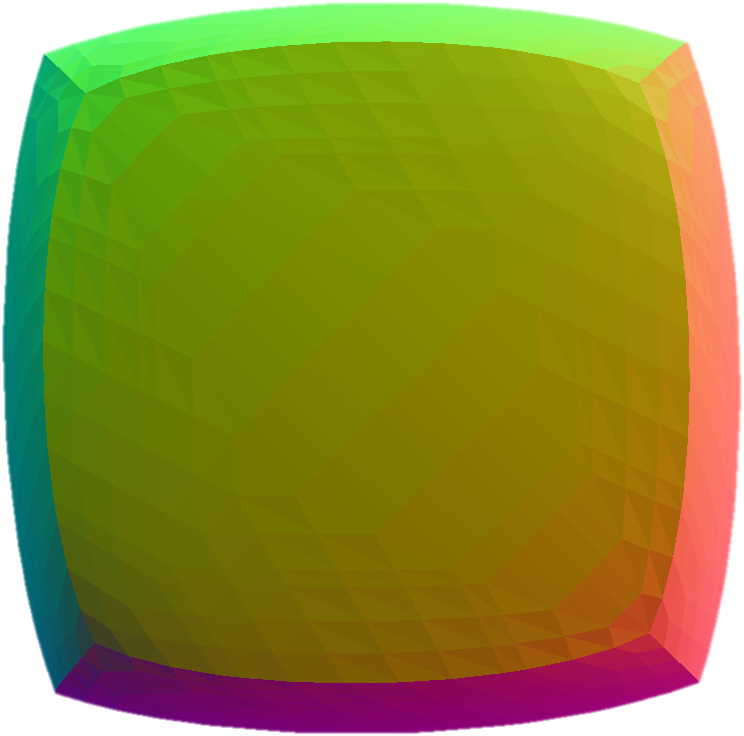
\includegraphics[width=\textwidth]{content/img/results/normals/cubeRealNormals.png}
		\caption{`Real' normals}
		\label{fig:results:normals:original:real}
	\end{subfigure}	
	\begin{subfigure}[t]{0.32\linewidth}
		\centering
		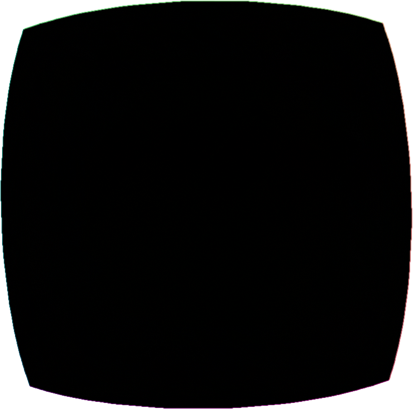
\includegraphics[width=\textwidth]{content/img/results/normals/cubeNormalsDifference.png}
		\caption{The difference between \subref{fig:results:normals:original:fake} and \subref{fig:results:normals:original:real}.}
		\label{fig:results:normals:original:difference}
	\end{subfigure}		
	\caption{A cube rendered with point-normal triangles colored according to the normalized normals, scaled to the open unit interval, using \subref{fig:results:normals:original:fake} fake and \subref{fig:results:normals:original:real} real normals. Both the inner and outer tessellation level were set to $12.0$. \Cref{fig:results:normals:original:difference} shows the difference between  using \subref{fig:results:normals:original:fake} a fake normal field or \subref{fig:results:normals:original:real} a real normal field.}
	\label{fig:results:normals:original}
\end{figure}

% \todo[inline]{Computational complexity of the fake normals and the real normals, consider one triangle.}
To compare the computational complexity we have counted the number of floating point operations (flops) required to determine the normal of one vertex on the rendered mesh, for both `fake' and `real' normals. 
% Fake normals
Evaluating the control net for the fake normal field for one vertex requires 23 flops. Computing the control net, which is not required for every vertex, requires 150 flops, i.e., if we consider the square roots necessary for the norm of the vectors in \crefe{eq:method:edge_coefficients} floating point operations for simplicity's sake. Consequently the number of flops required to compute $q$ vertices based on one input primitive is $150 + 23q$ flops.
% Real normals
If we count the floating point operations in \crefe{eq:method:normal:realNormal} we find that 59 flops are required to compute the `real' normal of one vertex. As a result the number of flops necessary to compute $q$ vertices based on one input primitive is $59q$. 
% Conclusion
Although order of the number of flops required to compute the normals of $q$ vertices is linear in $q$, the `fake' require less flops once a input triangle is tessellated into a shape that contains more than approximately five vertices. 

% \todo[inline]{Show results of PN triangles with fake and real normals, and discuss differences}
\Cref{fig:results:normals:original:fake} visualize the `fake' and `real' normal field of a cube. The difference image in \cref{fig:results:normals:original:difference} shows that these two normal fields are the same. A comparison of the `fake' and `real' normal field on other models did not reveal any difference either.  Thus we can conclude that the rendering is not influenced by the method used to compute the normals. 

% \todo[inline]{Iets zeggen over hoe kubussen pn triangles elkaar niet zo lief vinden}
Incidentally the cubes in \cref{fig:results:normals:original} illustrate one disadvantage of point-normal triangles, that is otherwise outside of the scope of this paper, namely that PN triangles are not suitable for rendering sharp edges. \Cref{fig:results:normals:original:fake,fig:results:normals:original:real} show how the originally sharp edges of the cube, become curved in a rendering with a high level of detail.